% PLEASE USE THIS FILE AS A TEMPLATE FOR THE PUBLICATION 
% Check file IOS-Book-Article.tex
%

\documentclass{IOS-Book-Article}     %[seceqn,secfloat,secthm]
%\usepackage{mathptmx}
%\usepackage[T1]{fontenc}
%\usepackage{times}%
\usepackage{graphicx}
\usepackage{amsmath}
\newtheorem{definition}{Definition}
%
%%%%%%%%%%% Put your definitions here
%IMPORTANT: ONLY INCLUDE AS %IMPORTANT: ONLY INCLUDE AS %IMPORTANT: ONLY INCLUDE AS \input{idp-latex/idp-latex-no-theorem}
\usepackage{import}

\subimport{idp-latex/}{includes-no-theorems}
\subimport{idp-latex/}{common-citations}




%The following are directives for LaTeX editors that collect ``included files'' to autocomplete macros etcetera
\ignore{
\include{includes-no-theorems}
\include{common-citations}
}
\usepackage{import}

\subimport{idp-latex/}{includes-no-theorems}
\subimport{idp-latex/}{common-citations}




%The following are directives for LaTeX editors that collect ``included files'' to autocomplete macros etcetera
\ignore{
\usepackage{ifthen}
\usepackage{url}
% \usepackage{cite} DOES NOT WORK WITH ALL STYLES
\usepackage{amssymb}
\usepackage{amsmath}
\usepackage{import}
\subimport{packages/}{xparse}
\usepackage{amsmath}
\usepackage[usenames,dvipsnames]{xcolor}
\usepackage{xspace}
\usepackage{datatool}
\usepackage{glossaries}

%ensured math mode with correct spacing
\providecommand\m[1]{\ensuremath{#1}\xspace}
\renewcommand{\m}[1]{\ensuremath{#1}\xspace}
\newcommand{\trval}[1]{\m{\mathbf{#1}}}



%%%%%%%%%%%%%%%%%%%%%%%%%%%%%%%%%%%%%%%%%%%%%%%%%%%%%%%%%%%%%%%%%%%%%%%%%%%%
%%%%%%%%%         LOGICAL STUFF: Operators, theories, ....         %%%%%%%%%
%%%%%%%%%%%%%%%%%%%%%%%%%%%%%%%%%%%%%%%%%%%%%%%%%%%%%%%%%%%%%%%%%%%%%%%%%%%%

%NOTE: arrows are not surrounded by the \m command. THe reason is that they are math operators that have
% other spacing 
% For instance: L\to L has spacing between L and \to and betwee \to and L, while L{\to}L does not. 

%% Logic
% lor, land, lnot are standard. Extensions:
	\newcommand{\limplies}{\Rightarrow}
	\newcommand{\limpl}{\limplies}
	\newcommand{\lequiv}{\Leftrightarrow}
	\newcommand{\limpliedby}{\Leftarrow}
	\newcommand{\limplied}{\limpliedby}
	\newcommand{\lrule}{\leftarrow}
	\newcommand{\cause}{\stackrel{c}{\lrule}}
	\newcommand{\rul}{\leftarrow}
	\newcommand{\ltrue}{\trval{t}}
	\newcommand{\lfalse}{\trval{f}}
	\newcommand{\lunkn}{\trval{u}}
	\newcommand{\lincon}{\trval{i}}
%related
	\newcommand{\bigand}{\bigwedge}
	\newcommand{\bigor}{\bigvee}
	\newcommand{\true}{\m{\top}}
	\newcommand{\false}{\m{\bot}}
% Marc zijn versies
	\newcommand{\Lra}{\Leftrightarrow}
	\newcommand{\lra}{\leftrightarrow}
	\newcommand{\Ra}{\Rightarrow}
	\newcommand{\La}{\Leftarrow}
	\newcommand{\ra}{\rightarrow}
	\newcommand{\la}{\leftarrow}
	\newcommand{\mim}{\limplies}
	\newcommand{\equi}{\lequiv}
	\newcommand{\Tr}{\ltrue}
	\newcommand{\Fa}{\lfalse}
	\newcommand{\Un}{\lunkn}
	\newcommand{\In}{\lincon}
	
%Vocabularies, structures, theories
	\newcommand{\voc}{\m{\Sigma}}
	\newcommand{\invoc}{\m{\sigma_{in}}}
	\newcommand{\outvoc}{\m{\sigma_{out}}}
	\newcommand{\struct}{\m{I}}
	\newcommand{\structx}{\m{I}}
	\newcommand{\I}{\m{\mathcal{I}}}
	\newcommand{\Iin}{\m{\I_{in}}}
	\newcommand{\J}{\m{\mathcal{J}}}
	\newcommand{\instruct}{\m{I_{in}}}
	\newcommand{\outstruct}{\m{I_{out}}}
	\newcommand{\theory}{\m{\mathcal{T}}}

%More caligraphic characters
	\newcommand{\PP}{\m{\mathcal{P}}}
	\newcommand{\LL}{\m{\mathcal{L}}}
	\newcommand{\WW}{\m{\mathcal{W}}}
	\newcommand{\BB}{\m{\mathcal{B}}}


%Often used abbreviations for definitions, formulas,...
	\newcommand{\D}{\m{\Delta}}
	\newcommand{\f}{\m{\varphi}}
	\newcommand{\atom}{\m{a}}
	\newcommand{\lit}{\m{l}}
	\newcommand{\rules}{\m{R}}
	\newcommand{\set}{\m{S}}
	\NewDocumentCommand\inter{g+g}{%
	  \IfNoValueTF{#1}
	    {\struct}
	    {\m{#1^{#2}}}}
	\newcommand{\partinter}{\m{J}}
	\newcommand{\model}{\m{M}}
	\newcommand{\fone}{\m{\varphi}}
	\newcommand{\ftwo}{\m{\psi}}

%properties of definitions
	\newcommand{\defined}[1]{\ensuremath{\mbox{\it Def}({#1})}\xspace}
	\newcommand{\open}[1]{\ensuremath{\mbox{\it Open}({#1})}\xspace}
	\newcommand{\pars}[1]{\ensuremath{\mbox{\it Par}({#1})}\xspace}
	\newcommand{\just}{\m{just}}

% Inferences
	\newcommand{\mx}[3]{\m{<#1, #2, #3>}}

%Vectors
	\newcommand{\xxx}{\m{\overline{x}}}
	\newcommand{\XXX}{\m{\overline{X}}}
	\newcommand{\yyy}{\m{\overline{y}}}
	\newcommand{\zzz}{\m{\overline{z}}}
	\newcommand{\ddd}{\m{\overline{d}}}
	\newcommand{\eee}{\m{\overline{e}}}
	\newcommand{\ccc}{\m{\overline{c}}}
	\newcommand{\bracketddd}{\m{\big(\overline{d}\big)}}
	\newcommand{\bddd}{\m{\big(\overline{d}\big)}}
	\newcommand{\DDD}{\m{\overline{D}}}
	\newcommand{\vvv}{\m{\overline{v}}}
	\newcommand{\ttt}{\m{\overline{t}}}
	\newcommand{\aaa}{\m{\overline{a}}}
	\newcommand{\bbb}{\m{\overline{b}}}
 	\providecommand{\lll}{\m{\overline{l}}}%sometimes, already exists
 	\renewcommand{\lll}{\m{\overline{l}}}
	\newcommand{\TTT}{\m{\overline{T}}}

%Set operations
	\newcommand{\elim}{\m{\backslash}}
	
%Rewrite rules
	\newcommand{\transformarrow}{\pmb{\pmb\rightarrowtail}}
	\newcommand{\rewrite}[2]{\m{#1  \ \transformarrow\    #2 }}

% Common Base types
	\newcommand{\bool}{\m{\mathbb{B}}}
	\newcommand{\Bool}{\bool}
	\newcommand{\nat}{\m{\mathbb{N}}}
	\newcommand{\Nat}{\nat}
	\renewcommand{\int}{\m{\mathbb{Z}}}
	\newcommand{\real}{\m{\mathbb{R}}}
	\newcommand{\rat}{\m{\mathbb{Q}}}

% Precision order
	\newcommand{\leqp}{\m{\leq_p}}
	\newcommand{\geqp}{\m{\geq_p}}
	\newcommand{\leqk}{\m{\leq_k}}
	\newcommand{\geqk}{\m{\geq_k}}
	\newcommand{\leqt}{\m{\leq_t}}
	\newcommand{\geqt}{\m{\geq_t}}
	
%Lattice operators
	\DeclareMathOperator\glb{glb}
	\DeclareMathOperator\lub{lub}
	\DeclareMathOperator\lfp{lfp}
	\DeclareMathOperator\gfp{gfp}


%valuations
	\newcommand{\val}{\m{\nu}}
	\newcommand{\superval}{\m{sv}}
	\newcommand{\kleeneval}{\m{Kl}}



%other
	\newcommand{\typed}[2]{\m{#1\in #2:}}
	\newcommand{\hasmodel}{\mid\!\equiv}
	\NewDocumentCommand\subs{g+g}{%
	  \IfNoValueTF{#1}
	    {\m{/}}
	    {\m{#1/ #2}}}
	\newcommand{\substitute}[2]{\subs{#1}{#2}}	
	\newcommand{\func}[1]{\m{f(#1)}}
	\newcommand{\setof}[1]{\m{\left \{ #1 \right \}}}
	\newcommand{\tuple}[1]{\m{\left \langle #1 \right \rangle }}
	\newcommand{\til}{\m{\sim}}
	\newcommand\eqdef{\mathrel{\overset{\makebox[0pt]{\mbox{\normalfont\tiny\sffamily def}}}{=}}}



%%%%%%%%%%%%%%%%%%%%%%%%%%%%%%%%%%%%%%%%%%%%%%%%%%%%%%%%%%%%%%%%%%%%%%%%%%%%
%%%%%%%%%                    Logics and systems                    %%%%%%%%%
%%%%%%%%%%%%%%%%%%%%%%%%%%%%%%%%%%%%%%%%%%%%%%%%%%%%%%%%%%%%%%%%%%%%%%%%%%%%

%General command to ensure correct spacing and text mode
	\newcommand{\logicname}[1]{\textsc{#1}\xspace}

%Systems
	\newcommand{\idp}{\logicname{IDP}}
	\newcommand{\xsb}{\logicname{XSB}}
	\newcommand{\idptwo}{\logicname{IDP$^2$}}
	\newcommand{\idpthree}{\logicname{IDP3}}
	\newcommand{\idpfour}{\logicname{IDP4}}
	\newcommand{\idpdraw}{\logicname{ID$^{P}_{Draw}$}}
	\newcommand{\idpide}{\logicname{ID$^{P}_{E}$}}
	\newcommand{\minisat}{\logicname{MiniSAT}}
	\newcommand{\minisatid}{\logicname{MiniSAT(ID)}}
	\newcommand{\gidl}{\logicname{GidL}}
	\newcommand{\sts}{\logicname{SAT-to-SAT}}
	\newcommand{\breakid}{\logicname{BreakID}}
	\newcommand{\glucose}{\logicname{Glucose}}
	\newcommand{\shatter}{\logicname{Shatter}}
	\newcommand{\saucy}{\logicname{Saucy}}
	\newcommand{\sbass}{\logicname{sbass}}
	\newcommand{\nauty}{\logicname{nauty}}
	\newcommand{\bliss}{\logicname{bliss}}
	\newcommand{\gringo}{\logicname{gringo}}
	\newcommand{\lparse}{\logicname{Lparse}}
	\newcommand{\smodels}{\logicname{Smodels}}
	

	
%logics
	\newcommand{\fodotidp}{\logicname{FO(\ensuremath{\cdot})\ensuremath{^{\mathtt{IDP}}}}}
	\newcommand{\foidp}{\fodotidp}
	\newcommand{\fodot}{\logicname{FO(\ensuremath{\cdot})}}
	\newcommand{\pcdot}{\logicname{PC(\ensuremath{\cdot})}}
	\newcommand{\foid}{\logicname{FO(ID)}}
	\newcommand{\foidaggpf}{\logicname{FO(ID,\allowbreak Agg,\allowbreak PF)}}
	\newcommand{\foidaggpft}{\logicname{FO(ID,\allowbreak Agg,\allowbreak PF,\allowbreak T)}}
	\newcommand{\foidplus}{\logicname{C-Log}} %DEPRECATED
	\newcommand{\clog}{\logicname{C-Log}}
	\newcommand{\foclog}{\logicname{FO(C)}}
	\newcommand{\hoid}{\logicname{HO(ID)}}
	\newcommand{\hopfid}{\logicname{HO(PF,ID)}}
	\newcommand{\fo}{\FO}
	\newcommand{\esoid}{\logicname{\ensuremath{\exists}SO(ID)}}
	\newcommand{\cpl}{\logicname{CP}-logic\xspace}
	\newcommand{\aspcore}{\text{\sc ASP-Core-2}\xspace}

%acronyms. USAGE: \ouracronym{CommandName}{A}{Acronym} creates a command \CommandName such that:
% * The first time you write it (probably the moment you define it), it reads Acronym (A)
% * All later times you use it, it simply says A.
% NOTE: to reset the counter, use \glsreset{<label>}
\newcommand{\ouracronym}[3]{%
	\newacronym{#1}{#2}{#3}
	\expandafter\newcommand\csname #1\endcsname{\gls{#1}\xspace}%
}
	\ouracronym{FO}{FO}{first-order logic}
	\ouracronym{PC}{PC}{propositional calculus}
	\ouracronym{MX}{MX}{Model Expansion}
	\ouracronym{MO}{MO}{Model Optimization}
	\ouracronym{ASP}{ASP}{Answer Set Programming}
	\ouracronym{TP}{TP}{Theorem Proving}
	\ouracronym{LP}{LP}{Logic Programming}
	\ouracronym{CP}{CP}{Constraint Programming}
	\ouracronym{FP}{FP}{Functional Programming}
	\ouracronym{KR}{KR}{Knowledge Representation}
	\ouracronym{CSP}{CSP}{Constraint Satisfaction Problem}
	\ouracronym{SMT}{SMT}{SAT Modulo Theories}
	\ouracronym{KBS}{KBS}{knowledge base system}
	\ouracronym{NNF}{NNF}{Negation Normal Form}
	\ouracronym{FNNF}{FNNF}{Flat Negation Normal Form}
	\ouracronym{DefNNF}{DefNNF}{Definition Negation Normal Form}
	\ouracronym{DEFNF}{DEFNF}{Definition Normal Form}
	\newcommand{\DEFNNF}{\DefNNF} %Was previously called like this. Keeping consistency
	\ouracronym{CDCL}{CDCL}{Conflict-Driven Clause-Learning}
	\ouracronym{WFS}{WFS}{Well-Founded Semantics}
	\ouracronym{LCG}{LCG}{Lazy Clause Generation}
	\ouracronym{AEL}{AEL}{Autoepistemic Logic}
	\ouracronym{OEL}{OEL}{Ordered Epistemic Logic}
	\ouracronym{AFT}{AFT}{Approximation Fixpoint Theory}

%%%%%%%%%%%%%%%%%%%%%%%%%%%%%%%%%%%%%%%%%%%%%%%%%%%%%%%%%%%%%%%%%%%%%%%%%%%%
%%%%%%%%%       DEFINITIONS: commands for writing definitions      %%%%%%%%%
%%%%%%%%%%%%%%%%%%%%%%%%%%%%%%%%%%%%%%%%%%%%%%%%%%%%%%%%%%%%%%%%%%%%%%%%%%%%

%%%%%%%%%%%%%%%%%%%%%%%%%%%%%%%%%%%%%
%   Stuff for (delayed) definitions   %
%%%%%%%%%%%%%%%%%%%%%%%%%%%%%%%%%%%%%

% The only commands you should use explicitly are:
%	* Environment ldef for a logical definition (should be used in mathmode)
%	* Environment ltheo for a logical theory (starts mathmode itself)
%	* \LRule defines a rule, usage \LRule{HEAD}{BODY}{OPTIONAL: DELAY}{OPTIONAL: CONSTRUCTION}
% 		---> Can be used inside a ldef or an align environment
%% USAGE EXAMPLE:
% \begin{ltheo}
% \lnot S(1) \\
% \exists x\typed{D}: P(x) \\
% \forall x\typed{D}: P(x) \limpl R(x)\\
% \begin{ldef}
% \LRule{\forall x\typed{D}: R(x)}{ Q(x) \lor S(x)}{delay}{construction} \\
% \LRule{\forall x\typed{D}: R(x)}{ Q(x) \lor S(x)}{delay}{construction} \\
% \LRule{\forall x\typed{D}: R(x)}{ Q(x) \lor S(x)}{delay}{construction} \\
% \LRule{\forall x\typed{D}: Q(x)}{ R(x)}
% \end{ldef}
% \end{ltheo}
%
% You can use these rules in an align environment as follows:
% \begin{align*}
% \LRule{\forall x\typed{D}: R(x)}{ Q(x) \lor S(x)}{delay}{construction} \\
% \LRule{\forall x\typed{D}: R(x)}{ Q(x) \lor S(x)}{delay}{construction} \\
% \LRule{Q}{ R(x)}
% \end{align*}

	\makeatletter
	\def\ifenv#1{
	\def\@tempa{#1}%
	\def\@ttempa{#1*}%
	\ifx\@tempa\@currenvir
	\expandafter\@firstoftwo
	\else
	\expandafter\@secondoftwo
	\fi
	}
	\makeatother

%Delayed definition rule. Usage: \ddrule{HEAD}{BODY}{DELAY}{CONSTRUCTION}
	\newcommand{\ddrule}[4]{\ensuremath{#1 \leftarrow #2 & \{#3\} & #4}}
%Non-delayed definition rule. Usage: \drule{HEAD}{BODY}
	\newcommand{\drule}[2]{\ensuremath{#1 & \leftarrow & #2}}

%Delayed align rule. Usage: \darule{HEAD}{BODY}{DELAY}{CONSTRUCTION}
	\newcommand{\darule}[4]{\ensuremath{#1 \leftarrow #2 & \{#3\} & #4}}
%Non-delayed align rule. Usage: \arule{HEAD}{BODY}
	\newcommand{\arule}[2]{\ensuremath{#1 \, &\leftarrow \, #2}}

	\newenvironment{ldef}{\left\{\begin{array}{l@{ \,}l@{\,}l}}{\end{array}\right\}}
	\newenvironment{ltheo}{\[\begin{array}{l}}{\end{array}\]\ignorespacesafterend}

	\newcommand{\LNDRule}[2]{
	\ifenv{array}
	{\drule{#1}{#2}}
	{ \ifenv{align}
		{\arule{#1}{#2}}
		{\ifenv{align*}
		{\arule{#1}{#2}}
		{ERROR: using LDRule in unsupported environment: \@currenvir}
		}
	}
	}

	\newcommand{\LDRule}[4]{
	\ifenv{array}
	{\ddrule{#1}{#2}{#3}{#4}}
	{ \ifenv{align}
		{\darule{#1}{#2}{#3}{#4}}
		{\ifenv{align*}
		{\darule{#1}{#2}{#3}{#4}}
		{ERROR: using LDRule in unsupported environment: \@currenvir}
		}
	}
	}

% NOTE: if getting strange errors on alignments, you probably forgot the ldef environment
	\NewDocumentCommand\LRule{m+g+g+g}{%
		\IfNoValueTF{#2}%
		{#1.&}{%
		\IfNoValueTF{#3}
		{\LNDRule{#1}{#2.}}
		{\LDRule{#1}{#2.}{#3}{#4}}%
		}
	}



%FOR COMPLEX RULES: with a c above the lrule...

	\NewDocumentCommand\CLRule{m+g}{%
	\ifenv{array}
	{\cdrule{#1}{#2}}
	{ \ifenv{align}
		{\carule{#1}{#2}}
		{\ifenv{align*}
			{\carule{#1}{#2}}
			{ERROR: using CLRule in unsupported environment: \@currenvir}
		}
	}
	}

	\NewDocumentCommand\carule{m+g}{%
		\IfNoValueTF{#2}
			{\ensuremath{#1.}}
			{\ensuremath{#1 \, &\cause \, #2}}}
	\NewDocumentCommand\cdrule{m+g}{%
		\IfNoValueTF{#2}
			{\ensuremath{#1.}}
			{\ensuremath{#1 & \cause & #2}}}
	



%%%%%%%%%%%%%%%%%%%%%%%%%%%%%%%%%%%%%%%%%%%%%%%%%%%%%%%%%%%%%%%%%%%%%%%%%%%%
%            Stuff for rules for state-changes in an algorithm             %
%%%%%%%%%%%%%%%%%%%%%%%%%%%%%%%%%%%%%%%%%%%%%%%%%%%%%%%%%%%%%%%%%%%%%%%%%%%%

% The only commands you should use explicitly are:
%	* Environment lprop for a set of state-changing rules
%	* \AlgoRule defines a propagation rule, usage \AlgoRule{Name}{Previous state}{New state}{Condition}
% The whole environment is in MATH mode by default, so use hbox to obtain normal text.

	\newcommand{\algrule}[4]{
	\hbox{{#1}:}& 
	\quad #2 ~\longrightarrow~ #3 
	\hbox{~ if } #4\\
	}

	\newenvironment{lprop}{\[\begin{array}{ll}}{\end{array}\]}

	\newcommand{\AlgoRule}[4]{
	\ifenv{array}
	{\algrule{#1}{#2}{#3}{#4}}
		{ERROR: using AlgoRule in unsupported environment: \@currenvir}
	}


\newcommand{\commentstyle}{\color{Gray}}



%%%%%%%%%%%%%%%%%%%%%%%%%%%%%%%%%%%%%%%%%%%%%%%%%%%%%%%%%%%%%%%%%%%%%%%%%%%%
%%%%%%%                    In-paper commentstyle                     %%%%%%%
%%%%%%%%%%%%%%%%%%%%%%%%%%%%%%%%%%%%%%%%%%%%%%%%%%%%%%%%%%%%%%%%%%%%%%%%%%%%

	\newcommand{\ignore}[1]{}

%Boolean to quickly disable all comments
	\newboolean{nocomments}
	\setboolean{nocomments}{false}

%Boolean to decide whether we put our name in margin or not
	\newboolean{commentmargin}
	\setboolean{commentmargin}{true}

%General comments
	\newcommand{\namedcomment}[3]{%
		\ifthenelse{\boolean{nocomments}}%
		{}%IF no comments, write nothing
		{%Otherwise
			\ifthenelse{\boolean{commentmargin}}%
				{ {\color{#3} \marginpar{\color{#3}\sc #2}#1}  }%Name in margin
				{  {\color{#3} {\sc #2}: #1}  }%Name not in margin
		}%
	}
	\newcommand{\mnamedcomment}[3]{\ifthenelse{\boolean{nocomments}}{}{{\marginpar{ \color{#3}{\sc #2}:#1}}}}

	\newcommand{\namedchange}[4]{\marginpar{\color{#4}\sc #3}\textcolor{#4}{#1}\textcolor{gray}{\st{#2}}}

%todo's
	\newcommand{\todo}[1]{\namedcomment{#1}{TODO}{blue}}
	\newcommand{\todonm}[1]{{\color{blue}\sc TODO} #1}
	\newcommand{\mtodo}[1]{\mnamedcomment{#1}{TODO}{blue}}
	\newcommand{\old}[1]{\namedcomment{#1}{OLD}{gray}}

%Personal comments (KRR):
	\newcommand{\bart}[1]{\namedcomment{#1}{bb}{red}}
	\newcommand{\mbart}[1]{\mnamedcomment{#1}{bb}{red}}
	\newcommand{\gerda}[1]{\namedcomment{#1}{gj}{orange}}
	\newcommand{\marc}[1]{\namedcomment{#1}{md}{orange}}
	\newcommand{\joost}[1]{\namedcomment{#1}{jv}{purple}}
	\newcommand{\bdc}[1]{\namedcomment{#1}{bdc}{OliveGreen}}
	\newcommand{\broes}[1]{\namedcomment{#1}{bdc}{OliveGreen}}
	\newcommand{\mbroes}[1]{\mnamedcomment{#1}{bdc}{OliveGreen}}
	\newcommand{\pieter}[1]{\namedcomment{#1}{pvh}{NavyBlue}}
	\newcommand{\maurice}[1]{\namedcomment{#1}{mb}{orange}}
	\newcommand{\ingmar}[1]{\namedcomment{#1}{id}{purple}}
	\newcommand{\matthias}[1]{\namedcomment{#1}{mvdh}{blue}}
	\newcommand{\mmaurice}[1]{\mnamedcomment{#1}{mb}{orange}}
	\newcommand{\jo}[1]{ \namedcomment{#1}{jo}{Fuchsia}}
	\newcommand{\joachim}[1]{ \namedcomment{#1}{jj}{Sepia}}
	\newcommand{\mjoachim}[1]{ \mnamedcomment{#1}{jj}{Sepia}}
	\newcommand{\tim}[2]{\namedcomment{#1}{tvde}{brown}}
	\usepackage{soul}
	\newcommand{\bartch}[2]{\namedchange{#1}{#2}{bb}{red}}
	\newcommand{\broesch}[2]{\namedchange{#1}{#2}{bdc}{OliveGreen}}
%Personal comments  (Collaborations):
	\newcommand{\pjs}[1]{\namedcomment{#1}{pjs}{orange}}
	\newcommand{\jan}[1]{\namedcomment{#1}{jvdb}{orange}}
	\newcommand{\jvt}[1]{\namedcomment{#1}{jvt}{orange}}
	\newcommand{\aw}[1]{\namedcomment{#1}{aw}{orange}}


%%%%%%%%%%%%%%%%%%%%%%%%%%%%%%%%%%%%%%%%%%%%%%%%%%%%%%%%%%%%%%%%%%%%%%%%%%%%
%%%%%%%                   Useful in-text commands                    %%%%%%%
%%%%%%%%%%%%%%%%%%%%%%%%%%%%%%%%%%%%%%%%%%%%%%%%%%%%%%%%%%%%%%%%%%%%%%%%%%%%

% \newcommand{\keyword}[2]{%
% 	\expandafter\newcommand\csname #1\endcsname{#2\xspace}%
% 	\expandafter\newcommand\csname #1s\endcsname{#2s\xspace}%
% 	\expandafter\newcommand\csname #1ness\endcsname{#2ness\xspace}%
% % 	\expandafter\newcommand\MakeUppercase{\csname #1\endcsname}{#2\xspace}%
% %	\expandafter\newcommand\csname\makefirstuc{#1}\endcsname{\makefirstuc{#2}\xspace}%
% %	\expandafter\newcommand\csname\makefirstuc{#1}\endcsname{\makefirstuc{#2}s\xspace}%
% }

\newcommand{\superscript}[1]{\ensuremath{^{\textrm{#1}}}}
\newcommand{\subscript}[1]{\ensuremath{_{\textrm{#1}}}}
\usepackage{etoolbox}

\newcommand\setcitation[2]{%
  \csdef{mycommoncitation#1}{#2}}
\newcommand\getcitation[1]{%
  \csuse{mycommoncitation#1}}

\setcitation{IDP}{WarrenBook/DeCatBBD14}
\setcitation{idp}{WarrenBook/DeCatBBD14}
\setcitation{fodot}{tocl/DeneckerT08}
\setcitation{foid}{tocl/DeneckerT08}
\setcitation{cplogic}{journal/tplp/VennekensDB10}
\setcitation{CPlogic}{journal/tplp/VennekensDB10}
\setcitation{CP}{Apt03}
\setcitation{cp}{Apt03}
\setcitation{EZCSP}{lpnmr/Balduccini11}
\setcitation{KR}{Baral:2003}
\setcitation{ASPComp2}{lpnmr/DeneckerVBGT09}
\setcitation{ASPComp3}{journals/tplp/CalimeriIR14}
\setcitation{ASPComp4}{conf/lpnmr/AlvianoCCDDIKKOPPRRSSSWX13}
\setcitation{ASPComp6}{jair/GebserMR17}
\setcitation{CPSupport}{ictai/DeCat13}
\setcitation{CPsupport}{ictai/DeCat13}
\setcitation{functionDetection}{iclp/DeCatB13}
\setcitation{fodot2asp}{DeneckerLTV12} %TODO replace by journal publication if one is publishedr
\setcitation{Tarskian}{DeneckerLTV12} %Same as the one above 
\setcitation{Inca}{iclp/DrescherW12}
\setcitation{csp2asp}{ijcai/DrescherW11}
\setcitation{DPLLT}{cav/GanzingerHNOT04}
\setcitation{AspInPractice}{synthesis/2012Gebser}
\setcitation{clasp}{ai/GebserKS12}
\setcitation{oclingo}{kr/GebserGKOSS12}
\setcitation{gringo}{lpnmr/GebserST07}
\setcitation{cmodels}{aaai/GiunchigliaLM04}
\setcitation{inputster}{tplp/Jansen13}
\setcitation{DLV}{tocl/LeonePFEGPS06}
\setcitation{LearningPaper}{TPLP/BruynoogheBBDDJLRDV} %TODO replace by published version
\setcitation{clog}{iclp/BogaertsVDV14} %TODO replace by journal publication if one is published
\setcitation{foc}{iclp/BogaertsVDV14}
\setcitation{FOC}{iclp/BogaertsVDV14}
\setcitation{inferenceClog}{ecai/BogaertsVDV14}
\setcitation{examplesClog}{nmr/BogaertsVDV14b} %TODO replace by better publication if possible
\setcitation{AFT}{DeneckerBV12}
\setcitation{KBS}{iclp/DeneckerV08}
\setcitation{KBS-invitedtalk}{jelia/Denecker16}
\setcitation{KBPE}{inap/DePooterWD11}
\setcitation{lazyGrounding}{jair/CatDBS15} 
\setcitation{LazyGrounding}{jair/CatDBS15} 
\setcitation{lazygrounding}{jair/CatDBS15} 
\setcitation{lazygroundingASP}{ijcai/BogaertsW18} 
\setcitation{ASP}{marek99stable}
\setcitation{satid}{sat/MarienWDB08}
\setcitation{lazyclausegeneration}{constraints/OhrimenkoSC09}
\setcitation{FP}{ACMCS/Hudak89}
\setcitation{GroundingWithBounds}{jair/WittocxMD10}
\setcitation{SAT}{faia/SilvaLM09}
\setcitation{LTC}{iclp/Bogaerts14}
\setcitation{SPSAT}{ictai/DevriendtBMDD12}
\setcitation{BreakID}{sat/DevriendtBBD16}
\setcitation{breakid}{sat/DevriendtBBD16}
\setcitation{LCG}{stuckeyLCG}
\setcitation{MiniZinc}{conf/cp/NethercoteSBBDT07}
\setcitation{minizinc}{conf/cp/NethercoteSBBDT07}
\setcitation{amadini}{cpaior/AmadiniGM13}
\setcitation{bootstrapping}{ngc/BogaertsJDJBD16}
\setcitation{Bootstrapping}{ngc/BogaertsJDJBD16}
\setcitation{GroundedFixpoints}{ai/BogaertsVD15}
\setcitation{PartialGroundedFixpoints}{ijcai/BogaertsVD15}
\setcitation{LogicBlox}{datalog/GreenAK12}
\setcitation{proB}{journals/sttt/LeuschelB08}
\setcitation{NaturalInductions}{KR/DeneckerV14} %TODO replace by journal publication if one is published
\setcitation{LP}{jacm/EmdenK76}
\setcitation{SMT}{faia/BarrettSST09}
\setcitation{AF}{ai/Dung95}
\setcitation{ADF}{kr/BrewkaW10}
\setcitation{af}{ai/Dung95}
\setcitation{adf}{kr/BrewkaW10}
\setcitation{ADFRevisited}{ijcai/BrewkaSEWW13}
\setcitation{adfrevisited}{ijcai/BrewkaSEWW13}
\setcitation{DefaultLogic}{ai/Reiter80}
\setcitation{DL}{ai/Reiter80}
\setcitation{AEL}{mo85}
\setcitation{minisat}{sat/EenS03}
\setcitation{completion}{adbt/Clark78}
\setcitation{wasp}{lpnmr/AlvianoDFLR13}
\setcitation{minisatid}{ictai/DeCat13}
\setcitation{lcg}{stuckeyLCG}
\setcitation{CEGAR}{jacm/ClarkeGJLV03}
\setcitation{cegar}{jacm/ClarkeGJLV03}
\setcitation{CuttingPlane}{or/DantzigFJ54}
\setcitation{kodkod}{tacas/TorlakJ07}
\setcitation{cdcl}{Marques-SilvaS99}
\setcitation{CDCL}{Marques-SilvaS99}
\setcitation{1UIP}{iccad/ZhangMMM01}
\setcitation{relevance}{ijcai/JansenBDJD16}
\setcitation{relevance-implementation}{aspocp/JansenBDJD16}
\setcitation{WFS}{GelderRS91}
\setcitation{wfs}{GelderRS91}
\setcitation{UnfoundedSet}{GelderRS91}
\setcitation{stablesemantics}{iclp/GelfondL88}
\setcitation{StableSemantics}{iclp/GelfondL88}
\setcitation{shatter}{Shatter}
\setcitation{sbass}{drtiwa11a}
\setcitation{lparsemanual}{url:lparse_manual}
\setcitation{AIC}{ppdp/FlescaGZ04}
\setcitation{templates}{tplp/DassevilleHJD15}
\setcitation{templates2}{iclp/DassevilleHBJD16}
\setcitation{sat-to-sat}{aaai/JanhunenTT16}
\setcitation{sat-to-sat-qbf}{bnp/BogaertsJT16}
\setcitation{sat-to-sat-QBF}{bnp/BogaertsJT16}
\setcitation{sat-to-sat-SO}{kr/BogaertsJT16}
\setcitation{XSB}{SwiW12}
\setcitation{KCmap}{jair/DarwicheM02}
\setcitation{TLA}{DBLP:books/aw/Lamport2002}
\setcitation{EventB}{BookAbrial2010}
\setcitation{MX}{MitchellTHM06}
\setcitation{MIP}{Sierksma96}
\setcitation{perefectmodel}{minker88/Przymusinski88}
\setcitation{SafeInductions}{ijcai/BogaertsVD17}
\setcitation{AIC}{ppdp/FlescaGZ04}
\setcitation{aic}{ppdp/FlescaGZ04}
\setcitation{alpha}{lpnmr/Weinzierl17}
\setcitation{omiga}{jelia/Dao-TranEFWW12}
\setcitation{gasp}{fuin/PaluDPR09}
\setcitation{asperix}{lpnmr/LefevreN09a}
\setcitation{CTL}{lop/ClarkeE81}
\setcitation{AFT-AIC}{ai/BogaertsC18}
\setcitation{UltimateApproximator}{DeneckerMT04}
\setcitation{KripkeKleene}{Fitting85}
\setcitation{AFT-HO}{corr/CharalambidisRS18} %TODO replace
\setcitation{HereThere}{Heyting30}
\setcitation{dAEL}{ijcai/HertumCBD16}
\setcitation{SDD}{ijcai/Darwiche11}
\setcitation{HEX}{ijcai/EiterIST05}
\setcitation{wADF}{aaai/BrewkaSWW18}
\setcitation{wADFfix}{corr/BrewkaSWW18}
\setcitation{}{}
\setcitation{}{}
\setcitation{}{}
\setcitation{}{}
\setcitation{}{}
\setcitation{}{}
\setcitation{}{}
\setcitation{}{}
\setcitation{}{}
\setcitation{}{}
\setcitation{}{}
\setcitation{}{}
\setcitation{}{}
  
 %Command for in case you want multiple citations in one, e.g., \cite{\refto{fodot},\refto{idp}}
 %Warning: no safety checks
\newcommand\refto[1]{%
      \getcitation{#1}}
      
 %usage: \mycite{key}, e.g., \mycite{fodot} results in \cite{tocl/DeneckerT08}
\newcommand\mycite[1]{%
      \ifcsname mycommoncitation#1\endcsname%
   \cite{\getcitation{#1}}%
  \else%
    \cite{#1}%
  \fi%
}	
  
   %usage: \mycite{key}, e.g., \mycite{fodot} results in \cite{tocl/DeneckerT08}
\newcommand\mycitet[1]{%
      \ifcsname mycommoncitation#1\endcsname%
   \citet{\getcitation{#1}}%
  \else%
    \citet{#1}
  \fi%
}	
  

}
\usepackage{import}

\subimport{idp-latex/}{includes-no-theorems}
\subimport{idp-latex/}{common-citations}




%The following are directives for LaTeX editors that collect ``included files'' to autocomplete macros etcetera
\ignore{
\usepackage{ifthen}
\usepackage{url}
% \usepackage{cite} DOES NOT WORK WITH ALL STYLES
\usepackage{amssymb}
\usepackage{amsmath}
\usepackage{import}
\subimport{packages/}{xparse}
\usepackage{amsmath}
\usepackage[usenames,dvipsnames]{xcolor}
\usepackage{xspace}
\usepackage{datatool}
\usepackage{glossaries}

%ensured math mode with correct spacing
\providecommand\m[1]{\ensuremath{#1}\xspace}
\renewcommand{\m}[1]{\ensuremath{#1}\xspace}
\newcommand{\trval}[1]{\m{\mathbf{#1}}}



%%%%%%%%%%%%%%%%%%%%%%%%%%%%%%%%%%%%%%%%%%%%%%%%%%%%%%%%%%%%%%%%%%%%%%%%%%%%
%%%%%%%%%         LOGICAL STUFF: Operators, theories, ....         %%%%%%%%%
%%%%%%%%%%%%%%%%%%%%%%%%%%%%%%%%%%%%%%%%%%%%%%%%%%%%%%%%%%%%%%%%%%%%%%%%%%%%

%NOTE: arrows are not surrounded by the \m command. THe reason is that they are math operators that have
% other spacing 
% For instance: L\to L has spacing between L and \to and betwee \to and L, while L{\to}L does not. 

%% Logic
% lor, land, lnot are standard. Extensions:
	\newcommand{\limplies}{\Rightarrow}
	\newcommand{\limpl}{\limplies}
	\newcommand{\lequiv}{\Leftrightarrow}
	\newcommand{\limpliedby}{\Leftarrow}
	\newcommand{\limplied}{\limpliedby}
	\newcommand{\lrule}{\leftarrow}
	\newcommand{\cause}{\stackrel{c}{\lrule}}
	\newcommand{\rul}{\leftarrow}
	\newcommand{\ltrue}{\trval{t}}
	\newcommand{\lfalse}{\trval{f}}
	\newcommand{\lunkn}{\trval{u}}
	\newcommand{\lincon}{\trval{i}}
%related
	\newcommand{\bigand}{\bigwedge}
	\newcommand{\bigor}{\bigvee}
	\newcommand{\true}{\m{\top}}
	\newcommand{\false}{\m{\bot}}
% Marc zijn versies
	\newcommand{\Lra}{\Leftrightarrow}
	\newcommand{\lra}{\leftrightarrow}
	\newcommand{\Ra}{\Rightarrow}
	\newcommand{\La}{\Leftarrow}
	\newcommand{\ra}{\rightarrow}
	\newcommand{\la}{\leftarrow}
	\newcommand{\mim}{\limplies}
	\newcommand{\equi}{\lequiv}
	\newcommand{\Tr}{\ltrue}
	\newcommand{\Fa}{\lfalse}
	\newcommand{\Un}{\lunkn}
	\newcommand{\In}{\lincon}
	
%Vocabularies, structures, theories
	\newcommand{\voc}{\m{\Sigma}}
	\newcommand{\invoc}{\m{\sigma_{in}}}
	\newcommand{\outvoc}{\m{\sigma_{out}}}
	\newcommand{\struct}{\m{I}}
	\newcommand{\structx}{\m{I}}
	\newcommand{\I}{\m{\mathcal{I}}}
	\newcommand{\Iin}{\m{\I_{in}}}
	\newcommand{\J}{\m{\mathcal{J}}}
	\newcommand{\instruct}{\m{I_{in}}}
	\newcommand{\outstruct}{\m{I_{out}}}
	\newcommand{\theory}{\m{\mathcal{T}}}

%More caligraphic characters
	\newcommand{\PP}{\m{\mathcal{P}}}
	\newcommand{\LL}{\m{\mathcal{L}}}
	\newcommand{\WW}{\m{\mathcal{W}}}
	\newcommand{\BB}{\m{\mathcal{B}}}


%Often used abbreviations for definitions, formulas,...
	\newcommand{\D}{\m{\Delta}}
	\newcommand{\f}{\m{\varphi}}
	\newcommand{\atom}{\m{a}}
	\newcommand{\lit}{\m{l}}
	\newcommand{\rules}{\m{R}}
	\newcommand{\set}{\m{S}}
	\NewDocumentCommand\inter{g+g}{%
	  \IfNoValueTF{#1}
	    {\struct}
	    {\m{#1^{#2}}}}
	\newcommand{\partinter}{\m{J}}
	\newcommand{\model}{\m{M}}
	\newcommand{\fone}{\m{\varphi}}
	\newcommand{\ftwo}{\m{\psi}}

%properties of definitions
	\newcommand{\defined}[1]{\ensuremath{\mbox{\it Def}({#1})}\xspace}
	\newcommand{\open}[1]{\ensuremath{\mbox{\it Open}({#1})}\xspace}
	\newcommand{\pars}[1]{\ensuremath{\mbox{\it Par}({#1})}\xspace}
	\newcommand{\just}{\m{just}}

% Inferences
	\newcommand{\mx}[3]{\m{<#1, #2, #3>}}

%Vectors
	\newcommand{\xxx}{\m{\overline{x}}}
	\newcommand{\XXX}{\m{\overline{X}}}
	\newcommand{\yyy}{\m{\overline{y}}}
	\newcommand{\zzz}{\m{\overline{z}}}
	\newcommand{\ddd}{\m{\overline{d}}}
	\newcommand{\eee}{\m{\overline{e}}}
	\newcommand{\ccc}{\m{\overline{c}}}
	\newcommand{\bracketddd}{\m{\big(\overline{d}\big)}}
	\newcommand{\bddd}{\m{\big(\overline{d}\big)}}
	\newcommand{\DDD}{\m{\overline{D}}}
	\newcommand{\vvv}{\m{\overline{v}}}
	\newcommand{\ttt}{\m{\overline{t}}}
	\newcommand{\aaa}{\m{\overline{a}}}
	\newcommand{\bbb}{\m{\overline{b}}}
 	\providecommand{\lll}{\m{\overline{l}}}%sometimes, already exists
 	\renewcommand{\lll}{\m{\overline{l}}}
	\newcommand{\TTT}{\m{\overline{T}}}

%Set operations
	\newcommand{\elim}{\m{\backslash}}
	
%Rewrite rules
	\newcommand{\transformarrow}{\pmb{\pmb\rightarrowtail}}
	\newcommand{\rewrite}[2]{\m{#1  \ \transformarrow\    #2 }}

% Common Base types
	\newcommand{\bool}{\m{\mathbb{B}}}
	\newcommand{\Bool}{\bool}
	\newcommand{\nat}{\m{\mathbb{N}}}
	\newcommand{\Nat}{\nat}
	\renewcommand{\int}{\m{\mathbb{Z}}}
	\newcommand{\real}{\m{\mathbb{R}}}
	\newcommand{\rat}{\m{\mathbb{Q}}}

% Precision order
	\newcommand{\leqp}{\m{\leq_p}}
	\newcommand{\geqp}{\m{\geq_p}}
	\newcommand{\leqk}{\m{\leq_k}}
	\newcommand{\geqk}{\m{\geq_k}}
	\newcommand{\leqt}{\m{\leq_t}}
	\newcommand{\geqt}{\m{\geq_t}}
	
%Lattice operators
	\DeclareMathOperator\glb{glb}
	\DeclareMathOperator\lub{lub}
	\DeclareMathOperator\lfp{lfp}
	\DeclareMathOperator\gfp{gfp}


%valuations
	\newcommand{\val}{\m{\nu}}
	\newcommand{\superval}{\m{sv}}
	\newcommand{\kleeneval}{\m{Kl}}



%other
	\newcommand{\typed}[2]{\m{#1\in #2:}}
	\newcommand{\hasmodel}{\mid\!\equiv}
	\NewDocumentCommand\subs{g+g}{%
	  \IfNoValueTF{#1}
	    {\m{/}}
	    {\m{#1/ #2}}}
	\newcommand{\substitute}[2]{\subs{#1}{#2}}	
	\newcommand{\func}[1]{\m{f(#1)}}
	\newcommand{\setof}[1]{\m{\left \{ #1 \right \}}}
	\newcommand{\tuple}[1]{\m{\left \langle #1 \right \rangle }}
	\newcommand{\til}{\m{\sim}}
	\newcommand\eqdef{\mathrel{\overset{\makebox[0pt]{\mbox{\normalfont\tiny\sffamily def}}}{=}}}



%%%%%%%%%%%%%%%%%%%%%%%%%%%%%%%%%%%%%%%%%%%%%%%%%%%%%%%%%%%%%%%%%%%%%%%%%%%%
%%%%%%%%%                    Logics and systems                    %%%%%%%%%
%%%%%%%%%%%%%%%%%%%%%%%%%%%%%%%%%%%%%%%%%%%%%%%%%%%%%%%%%%%%%%%%%%%%%%%%%%%%

%General command to ensure correct spacing and text mode
	\newcommand{\logicname}[1]{\textsc{#1}\xspace}

%Systems
	\newcommand{\idp}{\logicname{IDP}}
	\newcommand{\xsb}{\logicname{XSB}}
	\newcommand{\idptwo}{\logicname{IDP$^2$}}
	\newcommand{\idpthree}{\logicname{IDP3}}
	\newcommand{\idpfour}{\logicname{IDP4}}
	\newcommand{\idpdraw}{\logicname{ID$^{P}_{Draw}$}}
	\newcommand{\idpide}{\logicname{ID$^{P}_{E}$}}
	\newcommand{\minisat}{\logicname{MiniSAT}}
	\newcommand{\minisatid}{\logicname{MiniSAT(ID)}}
	\newcommand{\gidl}{\logicname{GidL}}
	\newcommand{\sts}{\logicname{SAT-to-SAT}}
	\newcommand{\breakid}{\logicname{BreakID}}
	\newcommand{\glucose}{\logicname{Glucose}}
	\newcommand{\shatter}{\logicname{Shatter}}
	\newcommand{\saucy}{\logicname{Saucy}}
	\newcommand{\sbass}{\logicname{sbass}}
	\newcommand{\nauty}{\logicname{nauty}}
	\newcommand{\bliss}{\logicname{bliss}}
	\newcommand{\gringo}{\logicname{gringo}}
	\newcommand{\lparse}{\logicname{Lparse}}
	\newcommand{\smodels}{\logicname{Smodels}}
	

	
%logics
	\newcommand{\fodotidp}{\logicname{FO(\ensuremath{\cdot})\ensuremath{^{\mathtt{IDP}}}}}
	\newcommand{\foidp}{\fodotidp}
	\newcommand{\fodot}{\logicname{FO(\ensuremath{\cdot})}}
	\newcommand{\pcdot}{\logicname{PC(\ensuremath{\cdot})}}
	\newcommand{\foid}{\logicname{FO(ID)}}
	\newcommand{\foidaggpf}{\logicname{FO(ID,\allowbreak Agg,\allowbreak PF)}}
	\newcommand{\foidaggpft}{\logicname{FO(ID,\allowbreak Agg,\allowbreak PF,\allowbreak T)}}
	\newcommand{\foidplus}{\logicname{C-Log}} %DEPRECATED
	\newcommand{\clog}{\logicname{C-Log}}
	\newcommand{\foclog}{\logicname{FO(C)}}
	\newcommand{\hoid}{\logicname{HO(ID)}}
	\newcommand{\hopfid}{\logicname{HO(PF,ID)}}
	\newcommand{\fo}{\FO}
	\newcommand{\esoid}{\logicname{\ensuremath{\exists}SO(ID)}}
	\newcommand{\cpl}{\logicname{CP}-logic\xspace}
	\newcommand{\aspcore}{\text{\sc ASP-Core-2}\xspace}

%acronyms. USAGE: \ouracronym{CommandName}{A}{Acronym} creates a command \CommandName such that:
% * The first time you write it (probably the moment you define it), it reads Acronym (A)
% * All later times you use it, it simply says A.
% NOTE: to reset the counter, use \glsreset{<label>}
\newcommand{\ouracronym}[3]{%
	\newacronym{#1}{#2}{#3}
	\expandafter\newcommand\csname #1\endcsname{\gls{#1}\xspace}%
}
	\ouracronym{FO}{FO}{first-order logic}
	\ouracronym{PC}{PC}{propositional calculus}
	\ouracronym{MX}{MX}{Model Expansion}
	\ouracronym{MO}{MO}{Model Optimization}
	\ouracronym{ASP}{ASP}{Answer Set Programming}
	\ouracronym{TP}{TP}{Theorem Proving}
	\ouracronym{LP}{LP}{Logic Programming}
	\ouracronym{CP}{CP}{Constraint Programming}
	\ouracronym{FP}{FP}{Functional Programming}
	\ouracronym{KR}{KR}{Knowledge Representation}
	\ouracronym{CSP}{CSP}{Constraint Satisfaction Problem}
	\ouracronym{SMT}{SMT}{SAT Modulo Theories}
	\ouracronym{KBS}{KBS}{knowledge base system}
	\ouracronym{NNF}{NNF}{Negation Normal Form}
	\ouracronym{FNNF}{FNNF}{Flat Negation Normal Form}
	\ouracronym{DefNNF}{DefNNF}{Definition Negation Normal Form}
	\ouracronym{DEFNF}{DEFNF}{Definition Normal Form}
	\newcommand{\DEFNNF}{\DefNNF} %Was previously called like this. Keeping consistency
	\ouracronym{CDCL}{CDCL}{Conflict-Driven Clause-Learning}
	\ouracronym{WFS}{WFS}{Well-Founded Semantics}
	\ouracronym{LCG}{LCG}{Lazy Clause Generation}
	\ouracronym{AEL}{AEL}{Autoepistemic Logic}
	\ouracronym{OEL}{OEL}{Ordered Epistemic Logic}
	\ouracronym{AFT}{AFT}{Approximation Fixpoint Theory}

%%%%%%%%%%%%%%%%%%%%%%%%%%%%%%%%%%%%%%%%%%%%%%%%%%%%%%%%%%%%%%%%%%%%%%%%%%%%
%%%%%%%%%       DEFINITIONS: commands for writing definitions      %%%%%%%%%
%%%%%%%%%%%%%%%%%%%%%%%%%%%%%%%%%%%%%%%%%%%%%%%%%%%%%%%%%%%%%%%%%%%%%%%%%%%%

%%%%%%%%%%%%%%%%%%%%%%%%%%%%%%%%%%%%%
%   Stuff for (delayed) definitions   %
%%%%%%%%%%%%%%%%%%%%%%%%%%%%%%%%%%%%%

% The only commands you should use explicitly are:
%	* Environment ldef for a logical definition (should be used in mathmode)
%	* Environment ltheo for a logical theory (starts mathmode itself)
%	* \LRule defines a rule, usage \LRule{HEAD}{BODY}{OPTIONAL: DELAY}{OPTIONAL: CONSTRUCTION}
% 		---> Can be used inside a ldef or an align environment
%% USAGE EXAMPLE:
% \begin{ltheo}
% \lnot S(1) \\
% \exists x\typed{D}: P(x) \\
% \forall x\typed{D}: P(x) \limpl R(x)\\
% \begin{ldef}
% \LRule{\forall x\typed{D}: R(x)}{ Q(x) \lor S(x)}{delay}{construction} \\
% \LRule{\forall x\typed{D}: R(x)}{ Q(x) \lor S(x)}{delay}{construction} \\
% \LRule{\forall x\typed{D}: R(x)}{ Q(x) \lor S(x)}{delay}{construction} \\
% \LRule{\forall x\typed{D}: Q(x)}{ R(x)}
% \end{ldef}
% \end{ltheo}
%
% You can use these rules in an align environment as follows:
% \begin{align*}
% \LRule{\forall x\typed{D}: R(x)}{ Q(x) \lor S(x)}{delay}{construction} \\
% \LRule{\forall x\typed{D}: R(x)}{ Q(x) \lor S(x)}{delay}{construction} \\
% \LRule{Q}{ R(x)}
% \end{align*}

	\makeatletter
	\def\ifenv#1{
	\def\@tempa{#1}%
	\def\@ttempa{#1*}%
	\ifx\@tempa\@currenvir
	\expandafter\@firstoftwo
	\else
	\expandafter\@secondoftwo
	\fi
	}
	\makeatother

%Delayed definition rule. Usage: \ddrule{HEAD}{BODY}{DELAY}{CONSTRUCTION}
	\newcommand{\ddrule}[4]{\ensuremath{#1 \leftarrow #2 & \{#3\} & #4}}
%Non-delayed definition rule. Usage: \drule{HEAD}{BODY}
	\newcommand{\drule}[2]{\ensuremath{#1 & \leftarrow & #2}}

%Delayed align rule. Usage: \darule{HEAD}{BODY}{DELAY}{CONSTRUCTION}
	\newcommand{\darule}[4]{\ensuremath{#1 \leftarrow #2 & \{#3\} & #4}}
%Non-delayed align rule. Usage: \arule{HEAD}{BODY}
	\newcommand{\arule}[2]{\ensuremath{#1 \, &\leftarrow \, #2}}

	\newenvironment{ldef}{\left\{\begin{array}{l@{ \,}l@{\,}l}}{\end{array}\right\}}
	\newenvironment{ltheo}{\[\begin{array}{l}}{\end{array}\]\ignorespacesafterend}

	\newcommand{\LNDRule}[2]{
	\ifenv{array}
	{\drule{#1}{#2}}
	{ \ifenv{align}
		{\arule{#1}{#2}}
		{\ifenv{align*}
		{\arule{#1}{#2}}
		{ERROR: using LDRule in unsupported environment: \@currenvir}
		}
	}
	}

	\newcommand{\LDRule}[4]{
	\ifenv{array}
	{\ddrule{#1}{#2}{#3}{#4}}
	{ \ifenv{align}
		{\darule{#1}{#2}{#3}{#4}}
		{\ifenv{align*}
		{\darule{#1}{#2}{#3}{#4}}
		{ERROR: using LDRule in unsupported environment: \@currenvir}
		}
	}
	}

% NOTE: if getting strange errors on alignments, you probably forgot the ldef environment
	\NewDocumentCommand\LRule{m+g+g+g}{%
		\IfNoValueTF{#2}%
		{#1.&}{%
		\IfNoValueTF{#3}
		{\LNDRule{#1}{#2.}}
		{\LDRule{#1}{#2.}{#3}{#4}}%
		}
	}



%FOR COMPLEX RULES: with a c above the lrule...

	\NewDocumentCommand\CLRule{m+g}{%
	\ifenv{array}
	{\cdrule{#1}{#2}}
	{ \ifenv{align}
		{\carule{#1}{#2}}
		{\ifenv{align*}
			{\carule{#1}{#2}}
			{ERROR: using CLRule in unsupported environment: \@currenvir}
		}
	}
	}

	\NewDocumentCommand\carule{m+g}{%
		\IfNoValueTF{#2}
			{\ensuremath{#1.}}
			{\ensuremath{#1 \, &\cause \, #2}}}
	\NewDocumentCommand\cdrule{m+g}{%
		\IfNoValueTF{#2}
			{\ensuremath{#1.}}
			{\ensuremath{#1 & \cause & #2}}}
	



%%%%%%%%%%%%%%%%%%%%%%%%%%%%%%%%%%%%%%%%%%%%%%%%%%%%%%%%%%%%%%%%%%%%%%%%%%%%
%            Stuff for rules for state-changes in an algorithm             %
%%%%%%%%%%%%%%%%%%%%%%%%%%%%%%%%%%%%%%%%%%%%%%%%%%%%%%%%%%%%%%%%%%%%%%%%%%%%

% The only commands you should use explicitly are:
%	* Environment lprop for a set of state-changing rules
%	* \AlgoRule defines a propagation rule, usage \AlgoRule{Name}{Previous state}{New state}{Condition}
% The whole environment is in MATH mode by default, so use hbox to obtain normal text.

	\newcommand{\algrule}[4]{
	\hbox{{#1}:}& 
	\quad #2 ~\longrightarrow~ #3 
	\hbox{~ if } #4\\
	}

	\newenvironment{lprop}{\[\begin{array}{ll}}{\end{array}\]}

	\newcommand{\AlgoRule}[4]{
	\ifenv{array}
	{\algrule{#1}{#2}{#3}{#4}}
		{ERROR: using AlgoRule in unsupported environment: \@currenvir}
	}


\newcommand{\commentstyle}{\color{Gray}}



%%%%%%%%%%%%%%%%%%%%%%%%%%%%%%%%%%%%%%%%%%%%%%%%%%%%%%%%%%%%%%%%%%%%%%%%%%%%
%%%%%%%                    In-paper commentstyle                     %%%%%%%
%%%%%%%%%%%%%%%%%%%%%%%%%%%%%%%%%%%%%%%%%%%%%%%%%%%%%%%%%%%%%%%%%%%%%%%%%%%%

	\newcommand{\ignore}[1]{}

%Boolean to quickly disable all comments
	\newboolean{nocomments}
	\setboolean{nocomments}{false}

%Boolean to decide whether we put our name in margin or not
	\newboolean{commentmargin}
	\setboolean{commentmargin}{true}

%General comments
	\newcommand{\namedcomment}[3]{%
		\ifthenelse{\boolean{nocomments}}%
		{}%IF no comments, write nothing
		{%Otherwise
			\ifthenelse{\boolean{commentmargin}}%
				{ {\color{#3} \marginpar{\color{#3}\sc #2}#1}  }%Name in margin
				{  {\color{#3} {\sc #2}: #1}  }%Name not in margin
		}%
	}
	\newcommand{\mnamedcomment}[3]{\ifthenelse{\boolean{nocomments}}{}{{\marginpar{ \color{#3}{\sc #2}:#1}}}}

	\newcommand{\namedchange}[4]{\marginpar{\color{#4}\sc #3}\textcolor{#4}{#1}\textcolor{gray}{\st{#2}}}

%todo's
	\newcommand{\todo}[1]{\namedcomment{#1}{TODO}{blue}}
	\newcommand{\todonm}[1]{{\color{blue}\sc TODO} #1}
	\newcommand{\mtodo}[1]{\mnamedcomment{#1}{TODO}{blue}}
	\newcommand{\old}[1]{\namedcomment{#1}{OLD}{gray}}

%Personal comments (KRR):
	\newcommand{\bart}[1]{\namedcomment{#1}{bb}{red}}
	\newcommand{\mbart}[1]{\mnamedcomment{#1}{bb}{red}}
	\newcommand{\gerda}[1]{\namedcomment{#1}{gj}{orange}}
	\newcommand{\marc}[1]{\namedcomment{#1}{md}{orange}}
	\newcommand{\joost}[1]{\namedcomment{#1}{jv}{purple}}
	\newcommand{\bdc}[1]{\namedcomment{#1}{bdc}{OliveGreen}}
	\newcommand{\broes}[1]{\namedcomment{#1}{bdc}{OliveGreen}}
	\newcommand{\mbroes}[1]{\mnamedcomment{#1}{bdc}{OliveGreen}}
	\newcommand{\pieter}[1]{\namedcomment{#1}{pvh}{NavyBlue}}
	\newcommand{\maurice}[1]{\namedcomment{#1}{mb}{orange}}
	\newcommand{\ingmar}[1]{\namedcomment{#1}{id}{purple}}
	\newcommand{\matthias}[1]{\namedcomment{#1}{mvdh}{blue}}
	\newcommand{\mmaurice}[1]{\mnamedcomment{#1}{mb}{orange}}
	\newcommand{\jo}[1]{ \namedcomment{#1}{jo}{Fuchsia}}
	\newcommand{\joachim}[1]{ \namedcomment{#1}{jj}{Sepia}}
	\newcommand{\mjoachim}[1]{ \mnamedcomment{#1}{jj}{Sepia}}
	\newcommand{\tim}[2]{\namedcomment{#1}{tvde}{brown}}
	\usepackage{soul}
	\newcommand{\bartch}[2]{\namedchange{#1}{#2}{bb}{red}}
	\newcommand{\broesch}[2]{\namedchange{#1}{#2}{bdc}{OliveGreen}}
%Personal comments  (Collaborations):
	\newcommand{\pjs}[1]{\namedcomment{#1}{pjs}{orange}}
	\newcommand{\jan}[1]{\namedcomment{#1}{jvdb}{orange}}
	\newcommand{\jvt}[1]{\namedcomment{#1}{jvt}{orange}}
	\newcommand{\aw}[1]{\namedcomment{#1}{aw}{orange}}


%%%%%%%%%%%%%%%%%%%%%%%%%%%%%%%%%%%%%%%%%%%%%%%%%%%%%%%%%%%%%%%%%%%%%%%%%%%%
%%%%%%%                   Useful in-text commands                    %%%%%%%
%%%%%%%%%%%%%%%%%%%%%%%%%%%%%%%%%%%%%%%%%%%%%%%%%%%%%%%%%%%%%%%%%%%%%%%%%%%%

% \newcommand{\keyword}[2]{%
% 	\expandafter\newcommand\csname #1\endcsname{#2\xspace}%
% 	\expandafter\newcommand\csname #1s\endcsname{#2s\xspace}%
% 	\expandafter\newcommand\csname #1ness\endcsname{#2ness\xspace}%
% % 	\expandafter\newcommand\MakeUppercase{\csname #1\endcsname}{#2\xspace}%
% %	\expandafter\newcommand\csname\makefirstuc{#1}\endcsname{\makefirstuc{#2}\xspace}%
% %	\expandafter\newcommand\csname\makefirstuc{#1}\endcsname{\makefirstuc{#2}s\xspace}%
% }

\newcommand{\superscript}[1]{\ensuremath{^{\textrm{#1}}}}
\newcommand{\subscript}[1]{\ensuremath{_{\textrm{#1}}}}
\usepackage{etoolbox}

\newcommand\setcitation[2]{%
  \csdef{mycommoncitation#1}{#2}}
\newcommand\getcitation[1]{%
  \csuse{mycommoncitation#1}}

\setcitation{IDP}{WarrenBook/DeCatBBD14}
\setcitation{idp}{WarrenBook/DeCatBBD14}
\setcitation{fodot}{tocl/DeneckerT08}
\setcitation{foid}{tocl/DeneckerT08}
\setcitation{cplogic}{journal/tplp/VennekensDB10}
\setcitation{CPlogic}{journal/tplp/VennekensDB10}
\setcitation{CP}{Apt03}
\setcitation{cp}{Apt03}
\setcitation{EZCSP}{lpnmr/Balduccini11}
\setcitation{KR}{Baral:2003}
\setcitation{ASPComp2}{lpnmr/DeneckerVBGT09}
\setcitation{ASPComp3}{journals/tplp/CalimeriIR14}
\setcitation{ASPComp4}{conf/lpnmr/AlvianoCCDDIKKOPPRRSSSWX13}
\setcitation{ASPComp6}{jair/GebserMR17}
\setcitation{CPSupport}{ictai/DeCat13}
\setcitation{CPsupport}{ictai/DeCat13}
\setcitation{functionDetection}{iclp/DeCatB13}
\setcitation{fodot2asp}{DeneckerLTV12} %TODO replace by journal publication if one is publishedr
\setcitation{Tarskian}{DeneckerLTV12} %Same as the one above 
\setcitation{Inca}{iclp/DrescherW12}
\setcitation{csp2asp}{ijcai/DrescherW11}
\setcitation{DPLLT}{cav/GanzingerHNOT04}
\setcitation{AspInPractice}{synthesis/2012Gebser}
\setcitation{clasp}{ai/GebserKS12}
\setcitation{oclingo}{kr/GebserGKOSS12}
\setcitation{gringo}{lpnmr/GebserST07}
\setcitation{cmodels}{aaai/GiunchigliaLM04}
\setcitation{inputster}{tplp/Jansen13}
\setcitation{DLV}{tocl/LeonePFEGPS06}
\setcitation{LearningPaper}{TPLP/BruynoogheBBDDJLRDV} %TODO replace by published version
\setcitation{clog}{iclp/BogaertsVDV14} %TODO replace by journal publication if one is published
\setcitation{foc}{iclp/BogaertsVDV14}
\setcitation{FOC}{iclp/BogaertsVDV14}
\setcitation{inferenceClog}{ecai/BogaertsVDV14}
\setcitation{examplesClog}{nmr/BogaertsVDV14b} %TODO replace by better publication if possible
\setcitation{AFT}{DeneckerBV12}
\setcitation{KBS}{iclp/DeneckerV08}
\setcitation{KBS-invitedtalk}{jelia/Denecker16}
\setcitation{KBPE}{inap/DePooterWD11}
\setcitation{lazyGrounding}{jair/CatDBS15} 
\setcitation{LazyGrounding}{jair/CatDBS15} 
\setcitation{lazygrounding}{jair/CatDBS15} 
\setcitation{lazygroundingASP}{ijcai/BogaertsW18} 
\setcitation{ASP}{marek99stable}
\setcitation{satid}{sat/MarienWDB08}
\setcitation{lazyclausegeneration}{constraints/OhrimenkoSC09}
\setcitation{FP}{ACMCS/Hudak89}
\setcitation{GroundingWithBounds}{jair/WittocxMD10}
\setcitation{SAT}{faia/SilvaLM09}
\setcitation{LTC}{iclp/Bogaerts14}
\setcitation{SPSAT}{ictai/DevriendtBMDD12}
\setcitation{BreakID}{sat/DevriendtBBD16}
\setcitation{breakid}{sat/DevriendtBBD16}
\setcitation{LCG}{stuckeyLCG}
\setcitation{MiniZinc}{conf/cp/NethercoteSBBDT07}
\setcitation{minizinc}{conf/cp/NethercoteSBBDT07}
\setcitation{amadini}{cpaior/AmadiniGM13}
\setcitation{bootstrapping}{ngc/BogaertsJDJBD16}
\setcitation{Bootstrapping}{ngc/BogaertsJDJBD16}
\setcitation{GroundedFixpoints}{ai/BogaertsVD15}
\setcitation{PartialGroundedFixpoints}{ijcai/BogaertsVD15}
\setcitation{LogicBlox}{datalog/GreenAK12}
\setcitation{proB}{journals/sttt/LeuschelB08}
\setcitation{NaturalInductions}{KR/DeneckerV14} %TODO replace by journal publication if one is published
\setcitation{LP}{jacm/EmdenK76}
\setcitation{SMT}{faia/BarrettSST09}
\setcitation{AF}{ai/Dung95}
\setcitation{ADF}{kr/BrewkaW10}
\setcitation{af}{ai/Dung95}
\setcitation{adf}{kr/BrewkaW10}
\setcitation{ADFRevisited}{ijcai/BrewkaSEWW13}
\setcitation{adfrevisited}{ijcai/BrewkaSEWW13}
\setcitation{DefaultLogic}{ai/Reiter80}
\setcitation{DL}{ai/Reiter80}
\setcitation{AEL}{mo85}
\setcitation{minisat}{sat/EenS03}
\setcitation{completion}{adbt/Clark78}
\setcitation{wasp}{lpnmr/AlvianoDFLR13}
\setcitation{minisatid}{ictai/DeCat13}
\setcitation{lcg}{stuckeyLCG}
\setcitation{CEGAR}{jacm/ClarkeGJLV03}
\setcitation{cegar}{jacm/ClarkeGJLV03}
\setcitation{CuttingPlane}{or/DantzigFJ54}
\setcitation{kodkod}{tacas/TorlakJ07}
\setcitation{cdcl}{Marques-SilvaS99}
\setcitation{CDCL}{Marques-SilvaS99}
\setcitation{1UIP}{iccad/ZhangMMM01}
\setcitation{relevance}{ijcai/JansenBDJD16}
\setcitation{relevance-implementation}{aspocp/JansenBDJD16}
\setcitation{WFS}{GelderRS91}
\setcitation{wfs}{GelderRS91}
\setcitation{UnfoundedSet}{GelderRS91}
\setcitation{stablesemantics}{iclp/GelfondL88}
\setcitation{StableSemantics}{iclp/GelfondL88}
\setcitation{shatter}{Shatter}
\setcitation{sbass}{drtiwa11a}
\setcitation{lparsemanual}{url:lparse_manual}
\setcitation{AIC}{ppdp/FlescaGZ04}
\setcitation{templates}{tplp/DassevilleHJD15}
\setcitation{templates2}{iclp/DassevilleHBJD16}
\setcitation{sat-to-sat}{aaai/JanhunenTT16}
\setcitation{sat-to-sat-qbf}{bnp/BogaertsJT16}
\setcitation{sat-to-sat-QBF}{bnp/BogaertsJT16}
\setcitation{sat-to-sat-SO}{kr/BogaertsJT16}
\setcitation{XSB}{SwiW12}
\setcitation{KCmap}{jair/DarwicheM02}
\setcitation{TLA}{DBLP:books/aw/Lamport2002}
\setcitation{EventB}{BookAbrial2010}
\setcitation{MX}{MitchellTHM06}
\setcitation{MIP}{Sierksma96}
\setcitation{perefectmodel}{minker88/Przymusinski88}
\setcitation{SafeInductions}{ijcai/BogaertsVD17}
\setcitation{AIC}{ppdp/FlescaGZ04}
\setcitation{aic}{ppdp/FlescaGZ04}
\setcitation{alpha}{lpnmr/Weinzierl17}
\setcitation{omiga}{jelia/Dao-TranEFWW12}
\setcitation{gasp}{fuin/PaluDPR09}
\setcitation{asperix}{lpnmr/LefevreN09a}
\setcitation{CTL}{lop/ClarkeE81}
\setcitation{AFT-AIC}{ai/BogaertsC18}
\setcitation{UltimateApproximator}{DeneckerMT04}
\setcitation{KripkeKleene}{Fitting85}
\setcitation{AFT-HO}{corr/CharalambidisRS18} %TODO replace
\setcitation{HereThere}{Heyting30}
\setcitation{dAEL}{ijcai/HertumCBD16}
\setcitation{SDD}{ijcai/Darwiche11}
\setcitation{HEX}{ijcai/EiterIST05}
\setcitation{wADF}{aaai/BrewkaSWW18}
\setcitation{wADFfix}{corr/BrewkaSWW18}
\setcitation{}{}
\setcitation{}{}
\setcitation{}{}
\setcitation{}{}
\setcitation{}{}
\setcitation{}{}
\setcitation{}{}
\setcitation{}{}
\setcitation{}{}
\setcitation{}{}
\setcitation{}{}
\setcitation{}{}
\setcitation{}{}
  
 %Command for in case you want multiple citations in one, e.g., \cite{\refto{fodot},\refto{idp}}
 %Warning: no safety checks
\newcommand\refto[1]{%
      \getcitation{#1}}
      
 %usage: \mycite{key}, e.g., \mycite{fodot} results in \cite{tocl/DeneckerT08}
\newcommand\mycite[1]{%
      \ifcsname mycommoncitation#1\endcsname%
   \cite{\getcitation{#1}}%
  \else%
    \cite{#1}%
  \fi%
}	
  
   %usage: \mycite{key}, e.g., \mycite{fodot} results in \cite{tocl/DeneckerT08}
\newcommand\mycitet[1]{%
      \ifcsname mycommoncitation#1\endcsname%
   \citet{\getcitation{#1}}%
  \else%
    \citet{#1}
  \fi%
}	
  

}

%%%%%%%%%%% End of definitions
\begin{document}

\newcommand{\Iota}{I}

\begin{frontmatter}          % The preamble begins here.
%
%\pretitle{}
\title{Using legal text in the knowledge base paradigm}
\runningtitle{}
%\subtitle{}

% For one author:
%\author{\fnms{} \snm{}}
%\address{}
%\runningauthor{}
%
% Two or more authors:
\author[A]{\fnms{Marjolein} \snm{Deryck}},
\author[B]{\fnms{Jo} \snm{Devriendt}}
\author[B]{\fnms{Simon} \snm{Marynissen}}
\author[A]{\fnms{Joost} \snm{Vennekens}}
\runningauthor{Deryck M. e.a.}
\address[A]{Department of Computer Science, KU Leuven, Campus De Nayer, Sint-Katelijne Waver, Belgium}
\address[B]{Department of Computer Science, KU Leuven, Leuven, Belgium}
%
\begin{abstract}
The Knowledge Base Paradigm advocates the accumulation of domain knowledge in a formal knowledge base to enable its use for multiple applications.
This practice induces flexibility and agility, as changes in the domain are reflected directly in the knowledge base, without affecting the algorithms that use this information.
Similarly, new ways to use this information can be developed independently of the specific domain and are highly portable.
This paper demonstrates these characteristics with the case of Belgian registration duties. 
The concerned legislation changed considerably mid 2018.  
Models for the former and current legislation are developed with IDP.
They are used in accordance with an interactive user interface for which a new implementation to interactively calculate and highlight relevant information was developed.
\end{abstract}


\begin{keyword}
Knowledge Base Paradigm, automatic configuration, IDP
\end{keyword}

\end{frontmatter}

%%%%%%%%%%% The article body starts:


\section{Introduction}

Legal applications have often been used as test cases for knowledge-based AI systems (e.g., \cite{cacm/SergotSKKHC86}). %, Zurek12}. %This was the case for traditional rule-based expert systems \cite{cacm/SergotSKKHC86}, but also for more recent systems such as, DROOLS \cite{Zurek12}. 
In \cite{ruleml/DeryckHVV18}, an interactive decision enactment system for notaries was developed according to the Knowledge Base Paradigm (KBP) \cite{iclp/DeneckerV08}. 

The KBP advocates a strict separation between declarative domain knowledge and the use of this knowledge to perform certain tasks. 
This separation allows the same knowledge to be used by different \emph{inference} algorithms in order to achieve different goals.
\begin{comment}
This is in contrast to  typical rule-based expert systems in which knowledge is formalized specifically with a forward-chaining inference algorithm in mind, or Prolog-based systems in which knowledge is formalized with a backwards query-answering algorithm in mind. 

In the KBP, domain knowledge is formalized as a purely declarative \emph{knowledge base}, which is not tied to a specific \emph{inference} method, allowing the same knowledge to be reused by different algorithms in order to achieve different goals.
\end{comment}
As claimed by \cite{iclp/DeneckerV08}, this paradigm has two main advantages. First, the knowledge base is easier to maintain, because it can be considered in isolation from the inference methods.  Second, the knowledge base is easier to reuse for other inference tasks, since it is not tied to any specific inference method anyway.

In \cite{ruleml/DeryckHVV18}, a decision enactment system that supports Belgian notaries in their handling of real estate sales was developed according to the KBP. The Belgian legislation on registration duties that need to be paid when purchasing real estate is quite complex: there exist multiple registration types with different rates, and legislation from the country's three regions may apply in addition to federal regulations. The tool was developed together with notary Luc Van Pelt. Like other Belgian notaries, his office prides itself on its customer-friendly and confidential service. Therefore, he is looking for a system that provides support while interviewing clients, without interrupting the natural flow of the conversation.% The system should therefore be able to accept relevant information in any order and to provide useful feedback  on each piece of information.

In this paper, we further analyze and develop the prototype that was developed in \cite{ruleml/DeryckHVV18}. This work focuses on validating the two advantages of the KBP mentioned above.
First, we update the prototype to cope with a recent change to Belgian legislation. This change was significant enough to warrant substantial coverage by major Belgian news outlets and therefore presents an interesting and representative test case for the maintainability of the knowledge base.
Second, during its evaluation of the prototype, the notary office identified additional desirable features that were not initially thought of. 
We were able to add these features to the prototype in a generic, domain-independent way. This supports the claim that the functionality that users desire can indeed be implemented by applying domain-independent inference methods to a purely declarative knowledge base, even if this functionality was not originally foreseen when the knowledge base was constructed.

This work results in a completely generic framework, similar to, but more powerful than that of \cite{ruleml/DassevilleJJVD16}. This generic framework can be applied to create powerful interactive decision enactment systems for other domains with minimal effort. It is developed using the \idp KBP system \mycite{IDP}, which allows it to benefit from both this system's expressive knowledge representation language \fodot, as well as from its efficient inference algorithms.
 
The next section elaborates on the background of the case, the main characteristics of the original prototype and the changes in legislation.
Section \ref{KBP} introduces the KBP and the \idp system.
%In Section \ref{original} the main characteristics of the original prototype are brought to mind.
Section \ref{interface} elaborates on new inferences in the revised interface.  
Section \ref{related} presents related work, followed by a discussion and conclusion in Section \ref{conclusion}.
\section{Method}
This case started in 2017, when the former legislation on registration duties was still applicable.
The use of Decision Model and Notation(DMN) was chosen as a methodology to analyze the applicable legislation and reflect it in connected decision tables \cite{DMN}. 
The main motivations to use DMN for this purpose are the availability and wide use of the open standard; and the proven integratability with IDP \cite{Ingmar}.
%After the analysis phase, the structured knowledge on the domain was translated to FO(.) for use in the Knowledge Base System (KBS) IDP \cite{IDP}.
For the application we use the IDP system, a state-of-the-art knowledge base system developed at KU Leuven \cite{IDP}.
In the IDP system the domain knowledge concerning registration duties is expressed in a rich, typed extension of First Order Logic to create a condensed knowledge base on the subject. 
It exists of a threefold structure.
A \textit{vocabulary} $\Sigma$ is a set of types, function and predicate symbols.
A \textit{theory } $T$ over $\Sigma$ is a set of sentences that expresses information on the domain in the form of constraints or definitions $\Delta$ and uses only symbols of $\Sigma$.
A \textit{structure} $I$ of $\Sigma$ represents a world.
It is an interpretation of (a part of) the vocabulary $\Sigma$ and associates functions and relations with their respective symbols.
A model $I$ of a theory T is an interpretation that satisfies all the sentences of T : $I \models T$.
For example, our application needs to select the appropriate tax rate to calculate the registration duty, depending on the registration type of the estate.
The vocabulary $\Sigma$ consist of types Rate and RegistrationType; and functions ApplicableRate:Rate and IsRegistrationType:RegistrationType.
Theory $T$ over $\Sigma$ consists of a definition of the applicable rate and the constraint that a rate should be specified:
\begin{center}
\[
\{
ApplicableRate = 10 \leftarrow IsRegistrationType = Other.
~\\
ApplicableRate = 1 \leftarrow IsRegistrationType = SocialDwelling.
~\\
ApplicableRate = 7 \leftarrow IsRegistrationType = FamilyDwelling.\}
~\\
\exists x : ApplicableRate = x.\]
\end{center}
The domain of Belgian registration duties is specified in the structure:\\
\[
Rate^I =& \{ 1,7,10\}\]~\\
\[RegistrationType^I =&\{Other,SocialDwelling,FamilyDwelling\}\]~\\


A variety of inferences can be applied to use this knowledge in applications.
With \textit{model expansion} IDP calculates an instance $J$ of the part of the vocabulary not covered by $I$ such that the two instances together satisfy theory $T$, or put differently: $I\cup J \models T$.
IDP can also \textit{optimize} instance $J$ for a given term.
By creating a term over $\Sigma$ of the form ${ min(\forall x, ApplicableRate = x, x)}$ and subsequently using the optimization inference on it, the model with the lowest applicable rate is calculated.
In our application the inferences of \textit{propagation} and \textit{relevance} are of main importance. 
%The more information is specified in structure $I$, the less free literals of vocabulary $\Sigma$ need to be determined in instance $J$, hence the less possible models remain.
Propagation is the calculation of the atoms from $\Sigma$ with respect to theory $T$ and based on the input information in $I$.
The inferences of relevance is discussed in length in section \ref{sec:relevance}.

As a user-friendly interface is of major importance to allow notaries and citizens to work with the application, the resulting knowledge base was used in combination with the existing interface from \cite{Ingmar}.
In the second run the existing models were adapted to the new legislation (applicable as from June 1st 2018) and new user requirements regarding the interface were incorporated in an enhanced user interface.




\section{Case study}
\subsection{Background}
\label{sec:background}
The legislation on registration duties was thoroughly reformed with the law of June 1st 2018. % check exacte naam wet
In the previous law most family houses would either be subject to the standard duty of 10\%, or to a reduced duty of 5\% for modest houses. 
To determine whether a house would classify as 'modest', the notion of \textit{cadastral income} was central.
It is a fictitious amount assigned to the house to represent the theoretical rental value of the house on reference date 01/01/1975.
Only for some houses this value got reviewed to current standards.
The \textit{cadastral income} was compared to a limit that depended on the number of children of the buyers.
On top of it, an elaborate system of \textit{abattement}(reductions on the taxable base of the house) with their own conditions existed.
In the new legislation that is in effect as from June 1st 2018 rules are simplified and the concept of \textit{cadastral income} was obliterated.
The system of \textit{abbatement} was abandoned and replaced by a fixed discount that follows the rules to determine the tax rate.
An overview model of the legislation prior and post June 2018 be found in Figure \ref{fig:DRD}.

%\begin{sidewaysfigure}
\begin{figure}[h]
    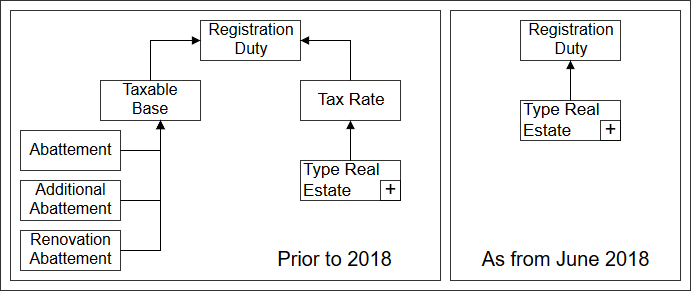
\includegraphics[angle=0,width = 0.8\linewidth]{img/A.png}
  	\caption{High-level structure of Belgian registration duties prior and post 1 June 2018.}
	\label{fig:DRD}
\end{figure}
%\end{sidewaysfigure}


\subsection{IDP theory}
\subsubsection{Regulation prior to June 1st 2018}
\label{sec:prior2018}
The initial analysis of the domain took a considerable amount of time, as the modeller did not have any prior domain knowledge.
Note that, especially with the approach used, the prior analysis of the domain and its formalization with the use of DMN could be done by a domain expert \cite{iets over DMN en gebruik door business users}.
However, some additional analysis and understanding of the domain by the IDP-modeller is needed, as some formulation choices impact the way variables are presented by the interface \cite{Marjolein}.

Typical for the former regulation was the use of multiple versions of the same concept at different law articles.
E.g., the definition of 'first property' and the establishment obligation were interpreted differently in the context of the type of real estate (TRE) and the context of \textit{abattement}.
%\begin{sidewaysfigure}
\begin{figure}[h]
    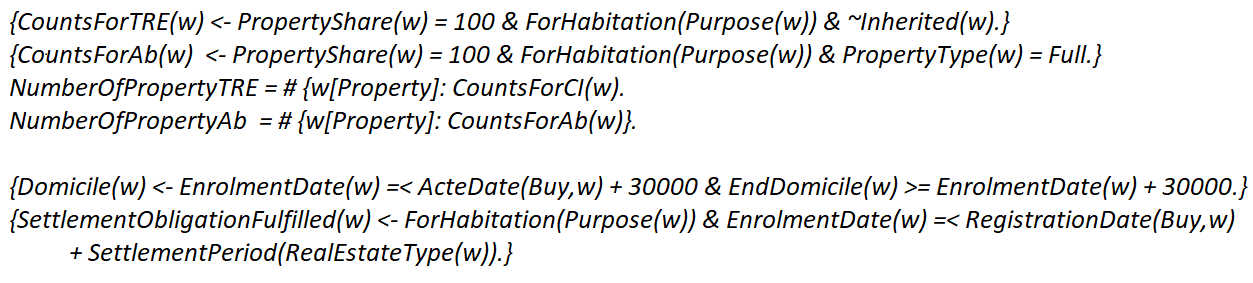
\includegraphics[angle=0,width = 1\linewidth]{img/codeOld.png}
  	%\caption{geen captation:voorbeeldcode.}
	\label{fig:code}
\end{figure}
%\end{sidewaysfigure}

The result is a large number of concepts, that also needs to be defined at a very fine-grained level to avoid confusion.
From an end-user point of view this creates an additional challenge to keep the interface clear.
In the original version the code was used with the interface proposed in \cite{Ingmar}.
Note that the IDP model of the registration duties did not have to be amended to use the functionality foreseen in this interface.
This demonstrates the distinction between the knowledge base and the inferences to use this information.
An important form of inference that is implemented by the interface is propagation.
This means that the consequences of the choice of the user are calculated, and if this results in an atom becoming certainly true or certainly false, these are highlighted in resp. green or red.%uitleggen in methode en daarnaar verwijzen%
This allows the end user to see the impact of his selections at a glance.
For a business expert, this offers a large advantage.
If a certain registration type has been derived to be impossible (i.e. highlighted in red), the notary knows that some other information does not have to be requested anymore, because as a business expert he knows that it is related to the registration type in question.
However, for naive end user, e.g. a first time buyer, it is not possible to know which information might still be relevant.
Moreover, both the chosen as the propagated selections appear in green and red, making it hard to see the difference between them (and hence, knowing which selection can be amended).

Another inference implemented by the interface is optimization. \jo{is it? Are we using Ingmar's version? Is there a split old regulations -> Ingmar's, new regulations -> Jo's? It's not terribly important to me, but would need to know :)}
At the end multiple combinations of \textit{abattement} and registration type might be possible, each leading to an other duty to be paid.
Typically buyers would prefer to use the option that minimizes this amount, and it can be selected by using the applicable inference in the interface.
As a final remark, the interface does not make a distinction between important, often used concepts and less used concepts.
All of the available concepts are shown in one screen, in the order of definition, which is a disadvantage given the large number of fine-grained concepts.

%%insert printscreen GUI

\subsubsection{Regulation as from June 1st 2018}
As discussed above, the regulation changed considerably as from June 1st 2018.
In our application we modelled the new regulation (without transitional measures for transactions concluded prior to June 1st but registered after this date).
One of the claims of KBP is that it allows agile adaptations, as all and only conditions are centralized in the concise knowledge base.
It took a half day of work to implement the profound changes that were described in \ref{sec:background}: two hours were needed to search, analyze and model the new legislation using DMN; and an additional hour and a half were needed to amend the IDP-code. %exacte timings opzoeken%
So after a short development period the new regulation is ready to be used in the existing interface.
However, because of the disadvantages mentioned in \ref{sec:prior2018} we decided to develop a new and easier interface.
In the new interface it is possible to give literals a priority code.
Only literals with priority code \textit{1} show up in the initial view, while literals with priority code \textit{2} are displayed when a user explicitly expands the view.
Literals can be given a label that may contain spaces.
Detailed explanation over literals can optionally be made available via information buttons.
Law text often contains very detailed definitions of concepts, that are known by experts.
To avoid confusion and enable use for less versed users, these fine-grained definitions needed to be modelled in the previous interface, leading to excess literals and code.
In the new interface, more abstract definitions with textual explanation suffice.
This led us to further simplify the knowledge base.
%add example%
Usability was further improved by the introduction of \emph{relevance}, a new form of inference that is discussed in section \ref{sec:relevance}.
The outlook of the interface was changed to make a clearer distinction between the choices made by the user and the propagated consequences, and an explanation was added to the latter, referring back to the choices that explain its propagation.
%iets bij zeggen over de tijd die het neemt om code op deze manier aan te passen?%
\jo{wel zeggen dat je er nu een .csv met extra info moet bijgeven}
\jo{wel geen modelexpansie of optimalisatie in de nieuwe versie. Moet ik die toevoegen?}
\jo{is het nodig om zo gedetailleerd te gaan? Verschil tussen twee gui's lijkt me minder belangrijk?}
\jo{misschien verwijzen naar Ingmars paper over de oude gui?}

\subsection{Relevance}
\label{sec:relevance}
In the previous paragraphs some of the difficulties and solutions to design a clear interface given the inherent complexity of legislation were discussed.
In this section we discuss the \emph{relevance} inference as an important aid to keep track of necessary parts of information.
The inference was developed for \idp{}'s internal search routines as described in \cite{Jansen2016}, but was not included in \idp{}'s external interface until now.

In a nutshell, relevance pinpoints the unassigned literals that can still contribute to satisfying a not yet satisfied constraint. In other words, all unassigned literals that have no possible impact on the truth value of any constraint are \emph{irrelevant}.

Consider the following extension to theory $T$ (and corresponding extension of vocabulary and structure) to define the registration type:
\begin{align*}
& \{ \\
& ~ IsRegistrationType = SocialDwelling \leftarrow Seller = LicencedSeller \\ 
& ~~ \wedge Purpose = SocialHabitation.\\
& ~ IsRegistrationType = FamilyDwelling \leftarrow BuyerType = NaturalPerson \wedge Price \leq Limit. \\
& ~ IsRegistrationType = Other \leftarrow IsRegistrationType \neq SocialDwelling \\
& ~~ \wedge IsRegistrationType \neq FamilyDwelling.\\
& \}\\
& \exists x \colon IsRegistrationType = x.
\end{align*}
\jo{Try to use natural mathematical symbols ("$\neg$" or "$\leq$") instead of IDP-specific stuff like "\~{}" or "$=<$"}

In case the estate has not been destined for social habitation ($Purpose \neq SocialHabitation$), the registration type cannot be \textit{SocialDwelling} anymore.
In other words, whether the \textit{Seller} is \textit{LicencedSeller}, is irrelevant. \jo{good example}
Similarly, if the Price of the dwelling is above a certain limit, the estate cannot be registered as a \textit{FamilyDwelling}, and the \textit{BuyerType} becomes irrelevant.
%%in praktijk na te kijken of dit ook zo in de interface aangegeven wordt!
% iets toe te voegen over constraint

The calculation of relevance is based on well-known justification theory (e.g.; \cite{Denecker93, Denecker2015}.
The direct justification of a literal gives a reason why this literal is true.
%Definition : For a domain literal $p$ \in $defs(\Delta)$ and s set $Jd$ of literals $l$ is a direct justification of a domain literal $p$
%Consider the literals l1 \ldots ln, p with $p$ \in $defs(\Delta)$ and defined by $p \leftarrow l1 \odot  \ldots  \odot ln$.  
Consider the literals $l$, $l_1$,.., $l_n$ and $p$ with $p=l$ or $p=\neg l$.\jo{Wat bedoel je met "$p=l$"? Je probeert ergens de notie van positieve of negatieve relevantie weer te geven? Misschien moeten wij het niet zo complex maken, aangezien de gui dit niet doet: een literal is relevant indien hij positief of negatief relevant is.}
\jo{ook: waarom met literals werken en niet met atomen?}
A set of literals $Jd$ is a direct justification of $p = l$:
if $p \leftarrow \neg l_1 \wedge \ldots \wedge l_n$ then $p = true$ if $Jd = \{l_1, \ldots ,l_n\}$;
if $p \leftarrow \neg l_1 \vee \ldots \vee l_n$ then $p=l$ if $Jd = \{l_i\}$ for some $i$.
A set of literals $Jd$ is a direct justification of $\neg p = l$:
if $p \leftarrow \neg l_1 \wedge \ldots \wedge l_n$ then $\neg p = l$ if $Jd = \{~l_i\}$ for some $i$;  
if $p \leftarrow \neg l_1 \vee \ldots \vee l_n$ then $\neg p = l$ if $Jd = \{\neg J_1,  \ldots , \neg J_n\}$.
A total justification $J$ for a literal $p$ contains its direct justifications and the direct justifications of $p$'s direct justifications.\jo{dus maar twee niveaus diep? Nee he, dit loopt door tot aan de opens, hoe diep ze ook zitten :)}
A path $\Pi$ is a sequence of direct justifications from the root to the bottom, i.e. to the point where the direct justification contains only parameter base literals.
For a given literal $p$ from theory $T$ multiple justification paths may be constructed.
They can be characterized by their truth order $f <_t u <_t t$ and their precision order  $u<_p f$ and $u<_p t$.
%A literal is irrelevant for $P$t if its value does not affect any justification for $Pt$\ref{Jansen2016}.
Instead of searching for a total interpretation $I$ of $T:\Sigma$ such that $I \models T$, the inference of relevance searches for a partial interpretation $I$ and a justification $J$ that justifies $p_T$ in $I$ \cite{Jansen2016}.
\begin{definition}
\label{def1}
\cite{Jansen2016}
Given a PC(ID) theory $T = \{p_T , \Delta \}$ and a partial interpretation $\Iota$, we define the set of relevant literals, denoted $R_T(I)$ as follows:
\begin{itemize}
    \item $p_T$ is relevant if $p_T$ is not justified,
    \item if $l \in R_T(I)$, $(l,l') \in dd_\Delta$ and $l'$ is not justified, then $l'$ is relevant.
\end{itemize}
\end{definition}
\jo{Moedige poging Marjolein, maar het ontbreekt aan structuur en duidelijkheid. Wat probeer je te definieren? Wat zijn de gegeven parameters van je definitie? Wat zijn de voorwaarden die onder de mogelijke configuraties van het gegevene een object vormen dat voldoet aan de definitie?}
\jo{Ik werk het later, maar je zag dit als een oefening. Het is je nog niet gelukt.}


\section{Related Work}
Simon
\section{Conclusion}
op te nemen in de conclusie:
- onze applicatie lost een praktijkprobleem op:
* zorgt ervoor dat enkel relevante info opgevraagd wordt
* notaris kan zeker zijn dat alle mogelijke kortingen gechecked worden
* tegelijk makkelijk in gebruik en weinig intrusief in bespreking met klanten

- demonstratie van relevantie in een praktijkcase
* werkt dit in praktijk even goed als wat we intuitief zouden verwachten?

- afzonderen van beslissingslogica in kennisbank werkt:
* snelle aanpassing van de logica bij veranderende regels
* geen extra inspanning om interface te gebruiken
* ontwikkeling van interface onafhankelijk van domeinprobleem dat beschreven is in de code.


%\bibliographystyle{splncs}
{\footnotesize\bibliography{bib.bib}}


%%%%%%%%%%% The bibliography starts:
\begin{thebibliography}{99}

\bibitem{Jansen2016}
Jansen, J., Bogaerts, B., Devriendt, J., Janssens, G.,  Denecker, M. (2016). Relevance for SAT(ID). Proceedings of the Twenty-Fifth International Joint Conference on Artificial Intelligence, 596~-~602.

\bibitem{Denecker2015}
Denecker, M., Brewka, G., Strass, H. (2015). A formal theory of justifications. In 13th International Conference on Logic Programming and Non-monotonic Reasoning (pp. 250–264). Springer.

\bibitem{Denecker93}
Denecker, M., \& De Schreye, D. (1993). Justification semantics: a unifying framework for the semantics of logic programs. In Proc. of the Logic Programming and Nonmonotonic Reasoning Workshop (pp. 365–379).

\bibitem{DMN}
OMG: Decision Model and Notation 1.1 (2016
\bibitem{IDP}
 de  Cat,  B.,  Bogaerts,  B.,  Bruynooghe,  M.,  Denecker,  M.:   Predicate  logic  as  a
modelling language: The IDP system.  CoRR
abs/1401.6312
(2014)
\bibitem{Ingmar}
Denecker, M., \& De Schreye, D. (1993). Justification semantics: a unifying framework for the semantics of logic programs. In Proc. of the Logic Programming and Nonmonotonic Reasoning Workshop (pp. 365–379).
\bibitem{Marjolein}
Deryck, Marjolein, Hasic, Faruk, Vanthienen, Jan, \& Vennekens, Joost. (accepted). A case based inquiry into the decision model and notation (DMN) and the knowledge base (KB) paradigm. Proceedings of RuleML RR 2018, Proceedings of RuleML RR 2018.


\end{thebibliography}
\end{document}

